\cvsection{Projects}

\descriptionstyle{
    Selection (not exhaustive) of some projects I've worked on that relate to my academic, professional, and personal interests.\\
    I consider them as way to experiment, learn, and get a hands-on approach to engineering.
}

\begin{cventries}

    %---------------------------------------------------------
    \cventry
    {Most of the projects were done individually, at the explicit request of the professor.}
    {Academic Projects}
    {Politecnico di Milano, Milan (IT) \& University of Waterloo, Waterloo (CA)}
    {14.09.2020 - PRESENT}
    {
        \begin{cvitems}
            \item {\textbf{Implementation of path planning algorithms}: memory-efficient graph and sample-based search algorithms (A*, Dijkstra, RRT, RRT* and RRT-Kinodynamic) for path planning in robotics. Implementation in MATLAB, validation on both 2D and 3D environments via ROS ecosystem.}
            \item {\textbf{Study on Nonreciprocal Behavior in Time-Space Modulated Beams}: analysis of diode-like behavior in time-space modulated beams by means of piezoelectric shunts. Structure simulations in Comsol Multiphysics, experimental data analysis with MATLAB.}
            \item {\textbf{Topology Optimization of Hub Carrier}: mass minimization of a hub carrier structure, with constraints on the compliance and the manufacturability. Analysis with Altair HyperWorks suite.}
            \item {\textbf{Modeling and Control of a MagLev system}: analysis of the dynamics of a magnetic levitation system, parameter identification and control/filters design (PID, LQR and MPC, coupled with KF and EKF). Simulation in MATLAB/Simulink and hardware deployment on \textit{RTDAC/PCI I/O} board from INTECO.}
            \item {\textbf{Topology Optimization of 2D structures}: implementation of optimization routines based on the CONLIN algorithm. Validation on both discrete and continuous problems.}
            \item {\textbf{Structural Health Monitoring (SHM) as a multivariate outlier detection problem}: analysis of a tie-rods element subjected to both damage and environmental variability, by means of statistical indices as Mahalanobis Squared Distance (MSD) and Principal Component Analysis (PCA).}
            \item {\textbf{Drag Coefficient Analysis of a Model Rocket Using Ansys Fluent}: simulation of the flow around a model rocket to determine the drag coefficient and comparison with theoretical model.}
            \item {\textbf{Development of a 2D CFD solver in C/C++ for the solution of the Navier-Stokes equations for incompressible flows}: implementation of the SCGS and SIMPLE algorithms, with validation on the lid-driven cavity flow.}
            \item {\textbf{Implementation of a nonlinear Finite Element Analysis (FEA) solver}: implementation of the plasticity theory based on the radial return algorithm on top of a linear FEA solver.}
            \item {\textbf{Chip Scale Atomic Clocks (CSAC)}: analysis of the physics behind their operation and current state of the art, with a focus on MEMS/NEMS technology.}
            \item {\textbf{Laser/Material Interaction}: thermal analysis of the laser cutting process, with a focus on the vaporization and melt mechanisms.}
            \item {\textbf{Analysis of the electronic density for a given molecule}: visualization of the electronic density field of a molecule using MATLAB.}
        \end{cvitems}
        \vspace{9pt}
        \begin{minipage}{\textwidth}
            \begin{minipage}{0.65\textwidth}
                \begin{equation*}
                    \begin{cases}
                        \dot{z} = v                                                                                                                                                                                                                                                                                   \\
                        \dot{v} = m^{-1} \left(\frac{1}{2} \frac{\partial L_1}{\partial z} I_1^2 + \frac{1}{2} \frac{\partial L_2}{\partial z} I_2^2 - \frac{1}{2} C_d A \rho \dot{z} |\dot{z}| + m g  \right)                                                                                                        \\
                        \dot{I_1} = \left( \frac{1}{2} \frac{\partial^2 L_1}{\partial I_1^2} I_1^2 + 2\frac{\partial L_1}{\partial I_1} I_1 + L_1 \right)^{-1} \left( -\frac{1}{2} \frac{\partial^2 L_1}{\partial I_1 \partial z} \dot{z} I_1^2 - \frac{\partial L_1}{\partial z} \dot{z} I_1 - R_1 I_1 + V_1 \right) \\
                        \dot{I_2} = \left( \frac{1}{2} \frac{\partial^2 L_2}{\partial I_2^2} I_2^2 + 2\frac{\partial L_2}{\partial I_2} I_2 + L_2 \right)^{-1} \left( -\frac{1}{2} \frac{\partial^2 L_2}{\partial I_2 \partial z} \dot{z} I_2^2 - \frac{\partial L_2}{\partial z} \dot{z} I_2 - R_2 I_2 + V_2 \right)
                    \end{cases}
                \end{equation*}
                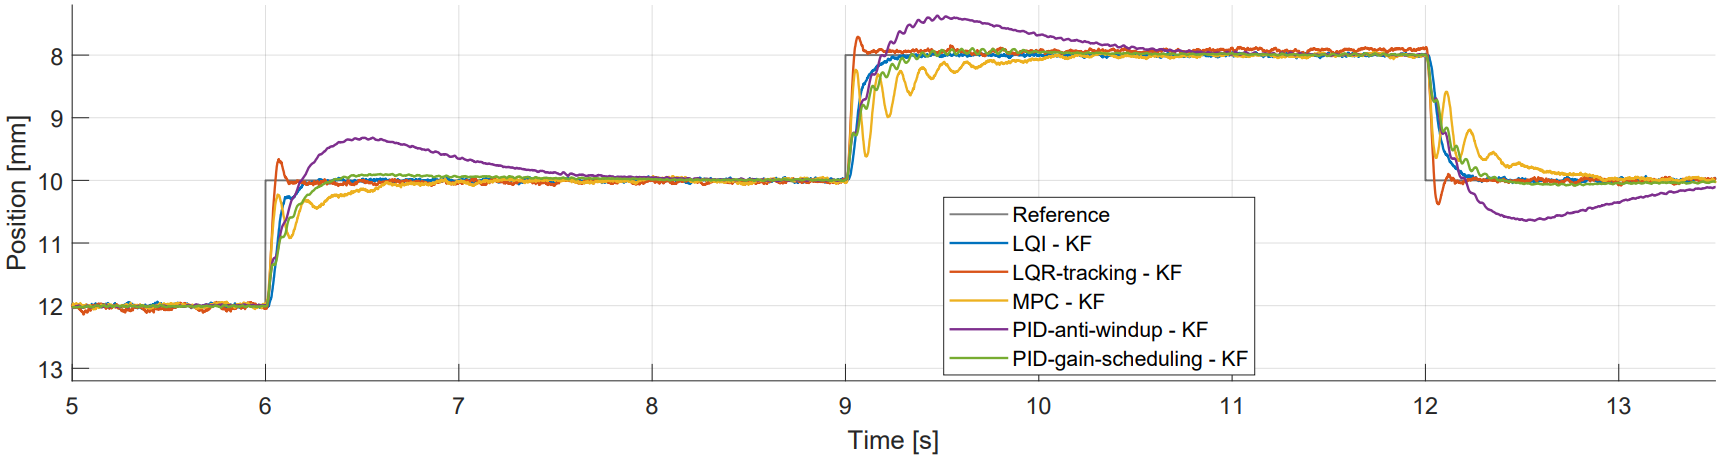
\includegraphics[width=0.95\textwidth]{common/img/Academic/2.png}
            \end{minipage}
            \hfill
            \begin{minipage}{0.33\textwidth}
                \vspace{9pt}
                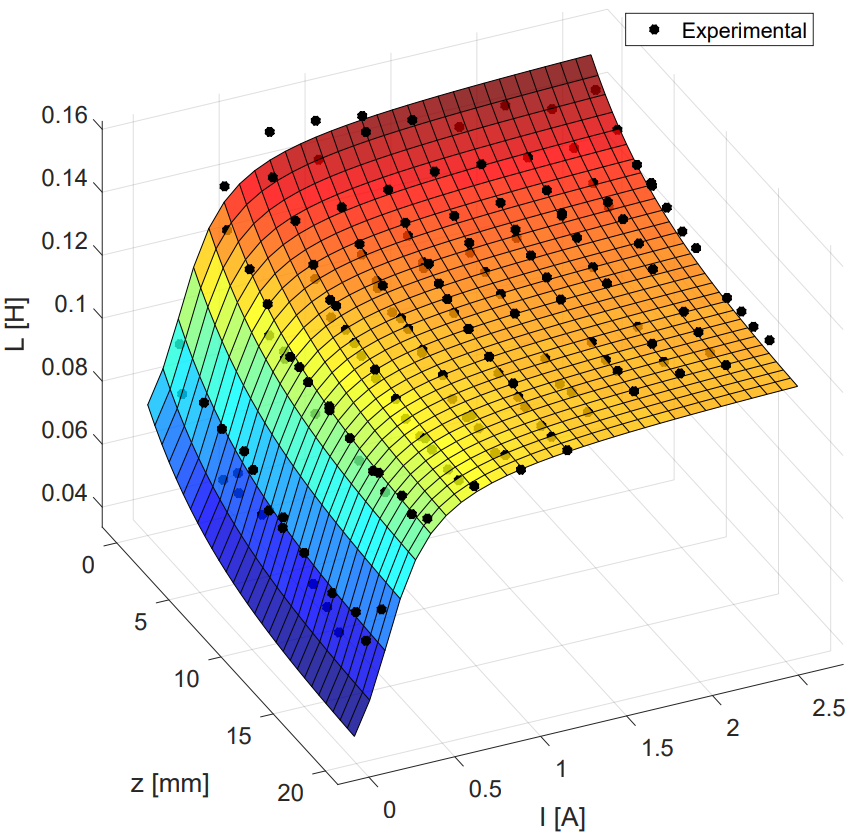
\includegraphics[width=\textwidth]{common/img/Academic/1.png}
            \end{minipage}
        \end{minipage}
        \begin{center}
            \vspace{5pt}
            \subdescriptionstyle{\textit{Extrapolated results from the MagLev project: system's equations of motion (top-left), inductance parameter identification (right) and system's response to a multistep input under different controllers (bottom-left). Accuracy of simulations allowed designing stable controllers in the full operability range of the system (3-22[mm]).}}
            \vspace{5pt}
        \end{center}
    }

    %---------------------------------------------------------
    \cventry
    {Pro Hackin' Project 2023, in partnership with RIMAC Automobili}
    {Personal Transportation Vehicle (Sidewalk vehicle)}
    {Politecnico di Milano, Milan (IT) \& RIMAC Automobili, Zagreb (HR)}
    {09.03.2023 - 01.06.2023}
    {
        \begin{minipage}{0.72\textwidth}
            \vspace{5pt}
            \begin{center}
                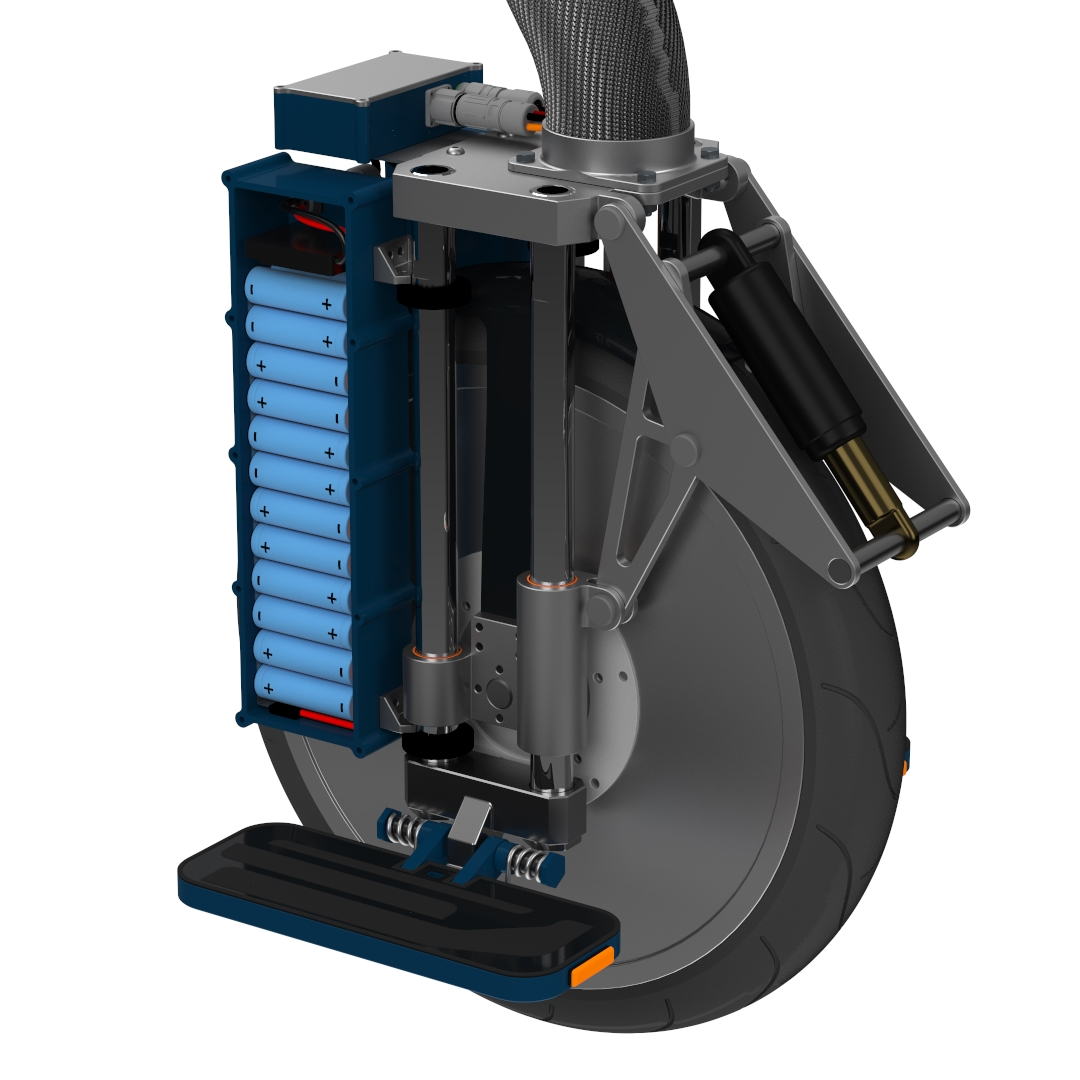
\includegraphics[height=120pt]{common/img/Rimac/1.jpg}
                \hspace{2cm}
                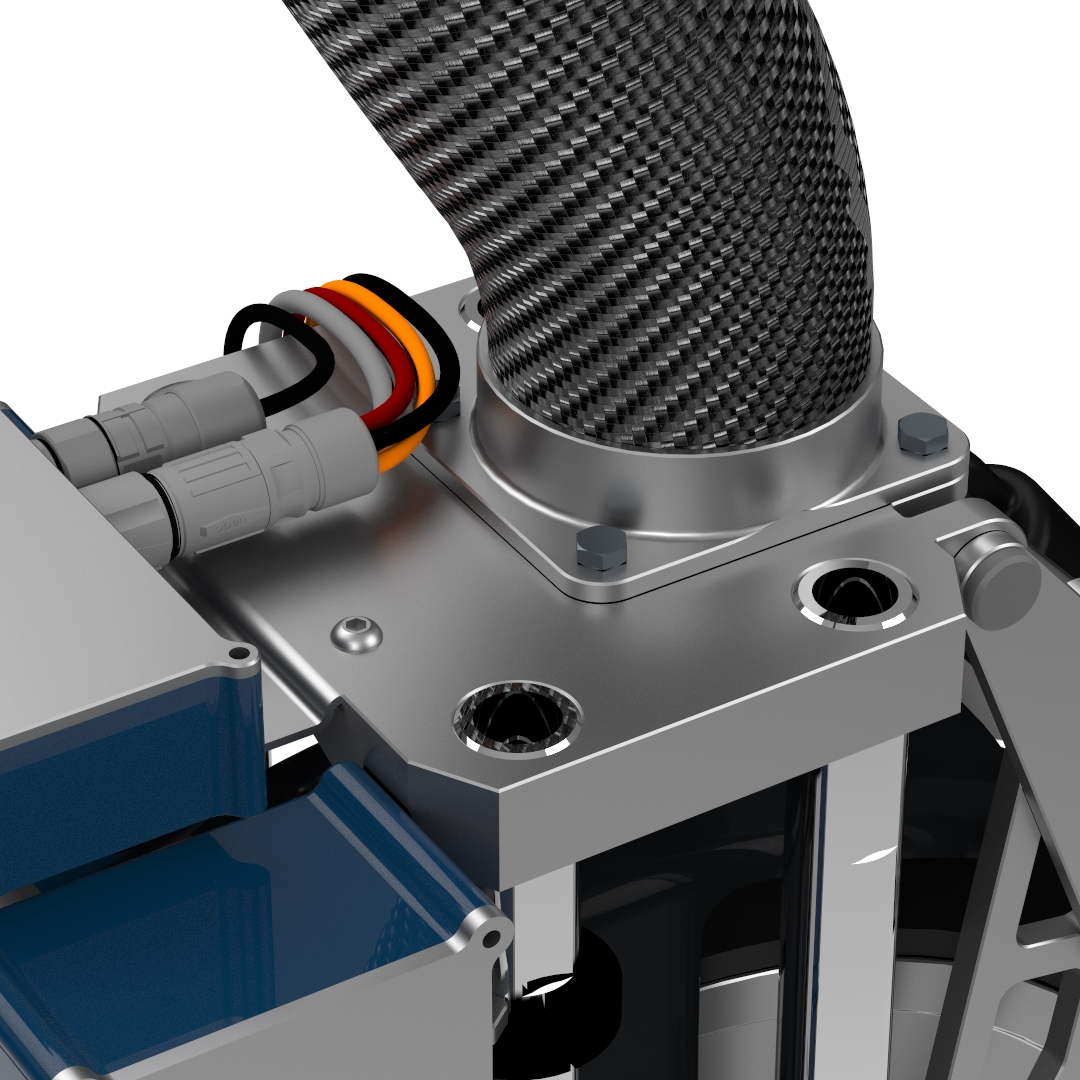
\includegraphics[height=120pt]{common/img/Rimac/2.jpg}
            \end{center}
            \vspace{5pt}
            Idealize and Design a Personal Transportation Vehicle (Sidewalk vehicle).\\
            Team-based project with students from 4 top European universities, featuring feedback sessions after each hackathon by company engineers. Selected as winning team.\\
            \begin{cvitems}
                \item {Hackathon 1: visions, user personas and functions \& requirements}
                \item {Hackathon 2: functional decomposition, morphological matrix and concepts development}
                \item {Hackathon 3: CAD design, FEM simulations, FMEA and cost analysis.}
            \end{cvitems}
            \vspace{4mm}
            \vspace{5pt}
        \end{minipage}
        \hfill
        \begin{minipage}{0.25\textwidth}
            \vspace{5pt}
            \begin{center}
                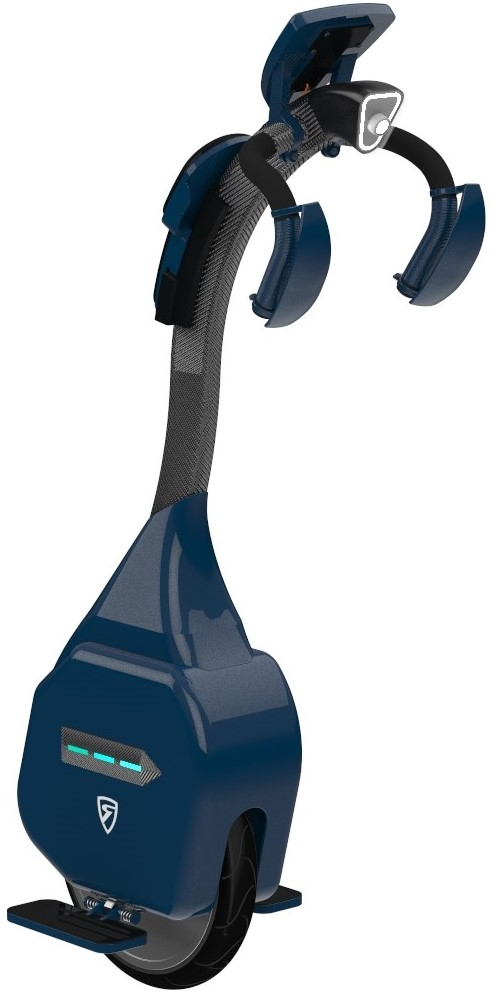
\includegraphics[height=200pt]{common/img/Rimac/3.jpg}
            \end{center}
            \vspace{5pt}
        \end{minipage}
    }

    %---------------------------------------------------------
    \cventry
    {Personal project to celebrate BSc}
    {Model Rocket with On-Board Flight Computer}
    {Personal Workshop, Como (IT)}
    {12.07.2023 - 21.07.2023}
    {
        \begin{minipage}{\textwidth}
            \vspace{5pt}
            \begin{overpic}[percent, width=\textwidth]{common/img/Rocket/Rocket.png}
                \put(4, 1.5){\subentrydatestyle{Fully functional flight computer in $< 20cm^3$}}
                \put(53, 1.5){\subentrydatestyle{Simulations driven design ($C_D \approx 0.806$)}}
                \put(19, 9.5){\subentrydatestyle{Launched and recovered without any damage, maximum elevation $+538m$}}
            \end{overpic}
            \vspace{3pt}
            Designing, optimization and building of a $63cm$ model rocket.\\
            Final design was achieved after a couple of iterations between CAD model and CFD simulations.
            Built mostly from cheap materials (cardboard \& wood) and 3D printed parts (PLA based).
            Essential characteristics:\\
            \begin{cvitems}
                \item {Flight time $\approx 60s$, maximum speed reached $+120m/s$, maximum acceleration $+10g$.}
                \item {Recovery system based on parachute, fully functional and reliable.}
                \item {On board flight computer with barometric, temperature and acceleration sensors capable of logging data.}
            \end{cvitems}
            \vspace{4mm}
        \end{minipage}
    }

    %---------------------------------------------------------
    \cventry
    {Done for fun or for educational purposes}
    {Selection of other minor projects}
    {Personal Workshop, Como (IT)}
    {2021 - PRESENT}
    {
        \begin{minipage}{0.45\textwidth}
            \vspace{5pt}
            \begin{center}
                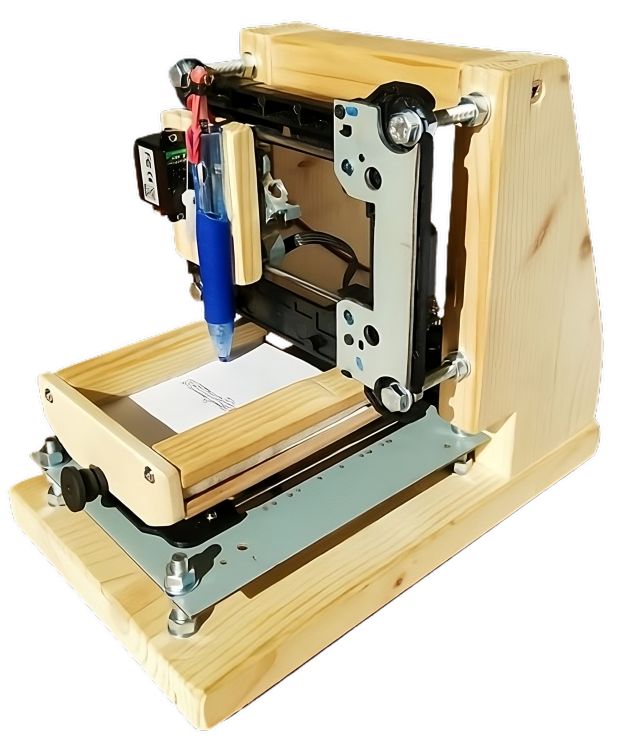
\includegraphics[height=150pt]{common/img/Minors/Gorlu.png}
                \hspace{4cm}
            \end{center}
            \vspace{5pt}
            CNC plotter to go from any digital image to its physical representation.\\
            \begin{cvitems}
                \item {Arduino based plotter with custom software.}
                \item {Canny edge detection algorithm.}
                \item {Recycled components from old DVD drives and wood.}
            \end{cvitems}
            \vspace{4mm}
            \vspace{5pt}
        \end{minipage}
        \hfill
        \begin{minipage}{0.45\textwidth}
            \vspace{5pt}
            \begin{center}
                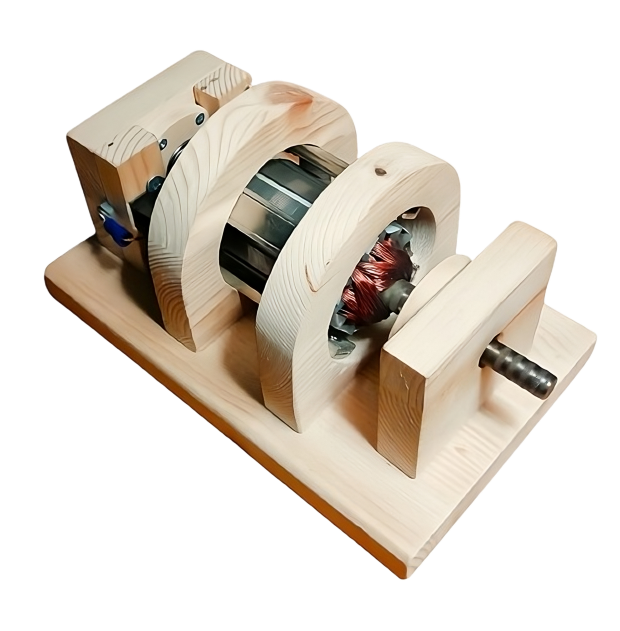
\includegraphics[height=150pt]{common/img/Minors/Joppo.png}
                \hspace{4cm}
            \end{center}
            \vspace{5pt}
            DC electric motor model to explain its working principle to my peer students.\\
            \begin{cvitems}
                \item {Recycled components from an old lawn mower and wood.}
                \item {Controllable in speed via a custom electrical circuit (diodes bridge and potentiometer).}
            \end{cvitems}
            \vspace{4mm}
            \vspace{5pt}
        \end{minipage}
    }

\end{cventries}